
\xiaosihao\songti
\begin{spacing}{1.5}
    \newpage
    \setcounter{page}{1}
    \pagenumbering{arabic}
    \section{绪论}
    
    \subsection{课题背景和选题意义}
    绪论部分主要论述选题的意义、国内外研究现状以及本文主要研究的内容、研究思路以及内容安排等。
    
    章标题为三号黑体加粗居中;一级节标题(如,2.1 本文研究内容):四号黑体居左;二级节标题(如,2.1.1 实验方法):小四号宋体居左。
    
    正文部分为小四号宋体,行间距1.5倍行距,首行缩进2个字符。
    
    \subsection{研究现状}
    \ldots
    \subsection{本文研究内容}
    \ldots
    \newpage
    \section{正文}
    
    正文部分每一章应另起页书写书写,层次要清楚,内容要有逻辑性,正文一般不少于15000字。正文部分因学科、选题特点可有差异,但必须言之成理,论据可靠,严格遵循本学科国际通行的学术规范。
    
    中文为小四号宋体,英文及数字为小四号Times New Roman,首行缩进2个字符,行间距为1.5倍。
    
    \subsection{插图格式要求}
    插图力求精炼,且每个插图均应有图序和图名。图序与图名位于插图下方,图序一般按章节编排,如图1-1(第一章第1个图),在插图较少时可以全文连续编序,如图10。

    如一个插图由两个及以上的分图组成,分图用(a)、(b)、(c)等标出,并标出分图名。

    简单文字图可用WORD直接绘制,复杂的图考虑使用相应的图形绘制软件完成,以提高图形表达质量。

    插图居中排列,与上文文本之间空一行。图序图名设置为五号宋体居中,图序与图名之间空一格。
    
    \begin{figure}[bhp]
        \centering
        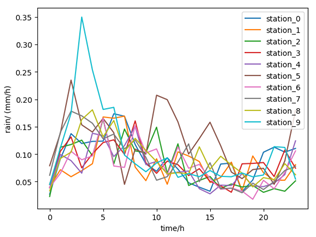
\includegraphics[scale=1]{figures/rainfall.png}
        \caption{\wuhao 每小时降水量24小时均值分布图}
        \label{rainfall}
    \end{figure}
    
    \begin{figure}
        \centering
        \begin{subfigure}{0.35\textwidth}
            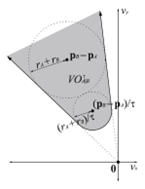
\includegraphics[width=3.83cm,height=5cm]{figures/speed-barrier-a.png}
            \subcaption{\wuhao 速度障碍集合}
        \end{subfigure}
        \begin{subfigure}{0.35\textwidth}
            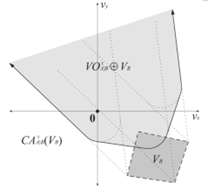
\includegraphics[height=5cm,width=5.51cm]{figures/speed-barrier-b.png}
            \subcaption{\wuhao 避免碰撞集合}
        \end{subfigure}
        \caption{\wuhao 速度障碍法速度选择}
        \label{speed}
    \end{figure}
    
    \subsection{表格格式要求}
    
    表格的结构应简洁,一律采用三线表,应有表序和表名,且表序和表名位于表格上方。表格可以逐章单独编序(如:表2.1),也可以统一编序(如:表10),采用哪种方式应和插图及公式的编序方式统一。表序必须连续,不得重复或跳跃。
    
    表格无法在同一页排版时,可以用续表的形式另页书写,续表需在表格右上角表序前加“续”字,如“续表2.1”,并重复表头。
    
    表格居中,边框为黑色直线1磅,中文为五号宋体,英文及数字为五号Times New Roman字体,表序与表名之间空一格,表格与下文之间空一行。
    
    
    \begin{table}
        \begin{center}
            \caption{测试表格}
            \begin{tabular}[c]{w{c}{0.3\linewidth}w{c}{0.3\linewidth}w{c}{0.3\linewidth}}
                \hline
                一 & 二 & 三\\
                \hline
                \ldots & \ldots &\ldots\\
                \ldots & \ldots &\ldots\\
                \ldots & \ldots &\ldots\\
                \ldots & \ldots &\ldots\\
                \hline
            \end{tabular}
        \end{center}
    \end{table}
    
    \subsection{表达式}
    
    论文中的公式应注序号并加圆括号,序号一律用阿拉伯数字连续编序(如(28))或逐章编序(如(3.6)),编号方式应与插图、表格方式一致。序号排在版面右侧,且距右边距离相等。公式与序号之间不加虚线。
    
    长公式在一行无法写完的情况下,原则上应在等号(或数学符号,如“+”、“-”号)处换行,数学符号在换行的行首。
    
    公式及文字中的一般变量(或一般函数)(如坐标X、Y,电压V,频率f)宜用斜体,矢量用粗斜体如S或白斜体上加单箭头,常用函数(如三角函数cos、对数函数ln等)、数字运算符、化学元素符号及分子式、单位符号、产品代号、人名地名的外文字母等用正体。
    
    公式排版时可选中模板中的“公式式样”,先将光标移至公式前,按“Tab”键,公式居中;再将光标移至编号前,按“Tab”键移动一个制表符位置,使公式编号右对齐。
    
    \begin{equation}
        V_{cell} = E_{OCV} - V_{act}- V_{ohm}- V_{horg}    
    \end{equation}
    
    \begin{equation}
        \begin{aligned}
            E_{OCV} &= 1.229-0.85\times 10^{-3}(T_{st}-T_0)\\
                    &+4.3085\times 10^{-5}T_{st}\left[\ln(\frac{P_{H_2}}{1.01325})+\frac{1}{2}\ln(\frac{P_{O_2}}{1.01325})\right]
        \end{aligned}
    \end{equation}
    
    \subsection{注释}
    
    正文中有个别名词或情况需要解释时,可加注说明,注释采用页末注(将注文放在加注页的下端)。在引文的右上角标注序号\footnote{这里本来应该有两个带圈数字的,不过我懒得加入Unicode支持了,反正正文也不出现这俩字符:)}……,如“马尔可夫链\footnote{ 马尔可夫链表示……}”。若在同一页中有两个以上的注时,按各注出现的先后,顺序编号。引文序号,以页为单位,且注释只限于写在注释符号出现的同页,不得隔页。
    注释采用小五号宋体,英文及数字为小五号Times New Roman字体,利用“引用”插入脚注功能插入。
    
    \newpage
    \section{总结与展望}
    
    \subsection{工作总结}
    最后一章结论与展望着重总结论文的创新点或新见解及研究展望或建议。
    
    结论是对论文主要研究结果、论点的提炼与概括,应准确、简明、完整、有条理,使人看后就能全面了解论文的意义、目的和工作内容。主要阐述自己的创造性工作及所取得的研究成果在本学术领域中的地位、作用和意义。
    
    结论要严格区分自己取得的成果与导师及他人的科研工作成果。在评价自己的研究工作成果时,要实事求是,除非有足够的证据表明自己的研究是“首次”的、“领先”的、“填补空白”的,否则应避免使用这些或类似词语。
    
    \subsection{工作展望}
    
    展望或建议,是在总结研究工作和现有结论的基础上,对该领域今后的发展方向及重要研究内容进行预测,同时对所获研究结果的应用前景和社会影响加以评价,从而对今后的研究有所启发。
        
\end{spacing}
